%!TEX root = ../main.tex
\chapter{Metodi iterativi per sistemi lineari}


L'idea di un metodo iterativo per la risoluzione di un sistema $A\x =\mathbf{b}$ è quella di costruire una successione di vettori
\begin{equation}
\x^{(0)} ,\x^{(1)} ,\x^{(2)} ,\dotsc ,\x^{(k)} \quad \text{tali che} \quad \x^{(k)}\xrightarrow{k\rightarrow \infty }\x.
\label{eq:idea-metodi-iterativi}
\end{equation}
Per ottenere tale risultato, dobbiamo saper rispondere a due questioni principali:
\begin{enumerate}
\item Come scegliere la successione di vettori in modo che \eqref{eq:idea-metodi-iterativi} sia verificata?
\item Come scegliere $k$ (dato che non possiamo svolgere infinite iterazioni) tale che $\left\Vert \x -\x^{(k)}\right\Vert < \operatorname{TOL}$, dove $\operatorname{TOL}$ è una tolleranza scelta dall'utente?
\end{enumerate}

La forma generale di un metodo iterativo è:
\begin{equation}
\text{Dato} \ \x^{(0)} ,\quad \x^{( k+1)} =B\x^{(k)} +\mathbf{g} ,\quad k \geqslant 0
\label{eq:forma-generale-metodo-iterativo}
\end{equation}
$B$ è detta \textbf{matrice di iterazione}\index{matrice!di iterazione} e dipende solo dalla matrice $A$, invece $\mathbf{g}$ può dipendere sia da $A$ che da $\mathbf{b}$.

Presentiamo ora due concetti molto importanti per la trattazione:
\begin{itemize}
\item \textbf{Convergenza:}
\begin{equation*}
\lim _{k\rightarrow \infty }\left\Vert \mathbf{e}^{(k)}\right\Vert = 0 \quad \text{con} \quad \mathbf{e}^{(k)} =\x -\x^{(k)} \quad k=0,1,2\dotsc
\end{equation*}
Per avere convergenza la successione degli errori deve tendere a zero, ricordando che vogliamo poter garantire tale risultato nonostante non conosciamo la soluzione esatta $\x$.
\item \textbf{Consistenza:}
\begin{equation*}
\x =B\x +\mathbf{g} \quad \left( \Rightarrow \mathbf{g} =( I-B) A^{-1}\mathbf{b}\right)
\end{equation*}
Se a un certo passo $k$ troviamo la soluzione esatta, il metodo deve restituire proprio quella.
In altre parole, la soluzione esatta deve soddisfare l'algoritmo, ovvero essa deve essere un punto fisso dell'algoritmo.
\end{itemize}

\textit{Controesempio.} La consistenza non implica la convergenza, come si vede scegliendo $B=I,\mathbf{g} =\mathbf{0}$:
\begin{equation*}
 \x =I\x +\mathbf{0} =\x \quad\text{(consistenza)},
\end{equation*}
ma
$$ \mathbf{\forall } k,\ \x^{( k+1)} =\x^{(k)} \ \ \Rightarrow \ \ \lim _{n\rightarrow \infty }\x^{(k)} = \x^{(0)} \neq \x. $$
A meno di non essere estremamente fortunati nella scelta di $\x^{(0)}$. \qedhere

Diamo ora un'importante definizione.
\begin{definition}
	[Residuo]
  \index{residuo}
  Sia dato un sistema lineare $A\x=\mathbf{b}$. Supponiamo di usare un metodo iterativo per la sua risoluzione e chiamiamo $\x^{(k)}$ il vettore della soluzione all'iterata $k$-esima. Definiamo residuo all'iterata $k$-esima la quantità
	\begin{equation}
		 \mathbf{r}^{(k)} =\mathbf{b} -A\x^{(k)}.
	\end{equation}
\end{definition}
Il residuo gioca un ruolo importante nel determinare quando è opportuno arrestare un metodo iterativo.
Idealmente vorremmo fissare un errore arbitrariamente piccolo, tuttavia dobbiamo farlo senza conoscere la soluzione esatta.
Ciò può apparentemente sembrare impossibile, ma vedremo degli opportuni criteri che garantiscono, ad esempio, che il residuo è una buona stima dall'alto dell'errore, in termini di norma. Chiederemo quindi che il residuo, che è una quantità calcolabile e nota ad ogni iterata, sia sufficientemente piccolo. Essendo inoltre tutte le norme non negative, potremo sostanzialmente applicare il teorema dei due carabinieri\footnote{Se $f(x)\le g(x)\le h(x),\ \forall x\in I$ e inoltre $f(x),h(x)\to l$ per $x\to x_{0} $, allora anche $g(x)\to l$ per $x\to x_{0}$.}:
\begin{equation*}
0\leqslant \underbrace{\left\Vert \mathbf{e}^{(k)}\right\Vert }_{\text{errore}} \leqslant \underbrace{\left\Vert \mathbf{r}^{(k)}\right\Vert =\left\Vert\mathbf{b} -A\x^{(k)}\right\Vert}_{\text{residuo}}\xrightarrow{k\rightarrow \infty } 0.
\end{equation*}
\begin{theorem}
Dato un metodo iterativo della forma \eqref{eq:forma-generale-metodo-iterativo} che sia consistente, si ha che:
\begin{equation*}
\text{convergenza} \ \ \Leftrightarrow \ \ \rho (B) < 1.
\end{equation*}
\end{theorem}
Possiamo sapere se il metodo converge semplicemente studiando il raggio spettrale di $B$. Chiedere che il raggio spettrale sia minore di $1$, significa chiedere che tutti gli autovalori stiano nel cerchio unitario. Si ha inoltre che se $\rho (B) \ll 1$ allora la convergenza è più veloce.

\textit{Dimostrazione.}
Al fine di dimostrare questo teorema, enunciamo la seguente proprietà: se $A\in \mathbb{R}^{n\times n}$,
\begin{equation}
A^{k}\xrightarrow{k\rightarrow \infty } 0\ \ \Leftrightarrow \ \ \rho (A) < 1.
\label{eq:prop-potenza-raggio-spettrale}
\end{equation}
Procediamo:
\begin{align*}
\x^{( k+1)} & =B\x^{(k)} +\mathbf{g} & \text{(metodo)}\\
\x & =B\x +\mathbf{g} & \text{(consistenza)}\\
\x -\x^{( k+1)} & =B(\x -\x^{(k)}) & \text{(sottraendo membro a membro)}\\
\mathbf{e}^{( k+1)} & =B\mathbf{e}^{(k)} . &
\end{align*}
Possiamo iterare l'equazione ottenuta per scriverla in funzione dell'errore al passo iniziale:
\begin{equation*}
\mathbf{e}^{(k)} =B\ \mathbf{e}^{( k-1)} =B\ \underbrace{B\ \mathbf{e}^{( k-2)}}_{\mathbf{e}^{( k-1)}} =\dotsc =B^{k}\mathbf{e}^{(0)}
\end{equation*}
Otteniamo dunque l'\textbf{equazione dell'errore}\index{equazione dell'errore}:
\begin{equation}
	\mathbf{e}^{(k)} =B^{k} \ \mathbf{e}^{(0)}
	\label{eq:equazione-errore}
\end{equation}
Dimostriamo ora i due versi della coimplicazione del teorema:
\begin{itemize}
\item $( \Rightarrow )$ usando nell'ultimo passaggio la proprietà \eqref{eq:prop-potenza-raggio-spettrale}:
\begin{equation*}
\underbrace{\mathbf{e}^{(k)}\xrightarrow{k\rightarrow \infty }\mathbf{0}}_{\text{convergenza}}  \ \ \Rightarrow \ \ B^{k}\xrightarrow{k\rightarrow \infty } 0\ \ \Rightarrow \ \ \rho (B) < 1
\end{equation*}
\item $( \Leftarrow )$ usando nel primo passaggio la proprietà \eqref{eq:prop-potenza-raggio-spettrale}:
\begin{equation*}
\rho (B) < 1 \ \ \Rightarrow \ \ B^{k}\xrightarrow{k\rightarrow \infty } 0\ \ \Rightarrow \ \ \underbrace{\mathbf{e}^{(k)}\xrightarrow{k\rightarrow \infty }\mathbf{0}}_{\text{convergenza}} . \qed
\end{equation*}
\end{itemize}
\section{Costruzione di metodi iterativi}

Vogliamo costruire un generico metodo iterativo della forma $\x^{( k+1)} =B\x^{(k)} +\mathbf{g}$, per risolvere il sistema $A\x =\mathbf{b}$.
\begin{enumerate}
\item Sia $P$ una matrice invertibile (ovvero con $\det(P) \neq 0$) detta \textbf{matrice di precondizionamento}\index{matrice!di precondizionamento}.
Dividiamo la matrice $A$ in due addendi:
\begin{equation*}
A=P-N.
\end{equation*}
\item Sostituiamo questa espressione nel sistema lineare:
\begin{align*}
A\x & =\mathbf{b}\\
( P-N)\x & =\mathbf{b}\\
P\x & =N\x +\mathbf{b}\\
\x & =\underbrace{P^{-1} N}_{B}\x +\underbrace{P^{-1}\mathbf{b}}_{\mathbf{g}}.
\end{align*}
\item Il metodo iterativo diventa, per $k\geqslant 0$:
\begin{equation}
\x^{( k+1)} =\underbrace{P^{-1} N}_{B}\x^{(k)} +\underbrace{P^{-1}\mathbf{b}}_{\mathbf{g}}.
\label{eq:forma-A-metodi-iterativi}
\end{equation}
o equivalentemente, dopo un po' di passaggi:
\begin{align*}
\x^{( k+1)} & =P^{-1} N\x^{(k)} +P^{-1}\mathbf{b}\\
\x^{( k+1)} & =P^{-1}( P-A)\x^{(k)} +P^{-1}\mathbf{b}\\
\x^{( k+1)} & =\left( I-P^{-1} A\right)\x^{(k)} +P^{-1}\mathbf{b}\\
\x^{( k+1)} & =\x^{(k)} -P^{-1} A\x^{(k)} +P^{-1}\mathbf{b}\\
\x^{( k+1)} & =\x^{(k)} +P^{-1}\left( -A\x^{(k)} +\mathbf{b}\right).
\end{align*}
In quest'ultima espressione riconosciamo i termini
\begin{equation}
	\x^{( k+1)} =\x^{(k)} +\overbrace{P^{-1}\underbrace{\left(\mathbf{b} -A\x^{(k)}\right)}_{\text{residuo} \ \mathbf{r}^{(k)}}}^{\mathbf{z}^{(k)}}.
	\label{eq:forma-B-metodi-iterativi}
\end{equation}
\end{enumerate}

\textit{Osservazioni.}
\begin{itemize}
\item $P$ caratterizza un metodo con questa forma; quindi è sufficiente scegliere $P$ per ottenere il metodo.
\item Un metodo così costruito è automaticamente consistente per costruzione, poiché lo abbiamo ottenuto a partire da $A\x =\mathbf{b}$.
\item Per calcolare $P^{-1}\mathbf{r}^{(k)}$, non serve calcolare l'inversa\footnote{In generale, l'inversione di matrice è un'operazione dispendiosa e potenzialmente instabile dal punto di vista numerico, quindi si cerca di utlizzarla il meno possibile, preferendo risoluzioni di sistemi lineari come nell'esempio appena mostrato.}, bensì basta risolvere il sistema $P\mathbf{z}^{(k)} =\mathbf{r}^{(k)}$, la cui soluzione $\mathbf{z}^{(k)}$ prende il nome di \textbf{residuo precondizionato}\index{residuo!precondizionato}.
Ovviamente risolvere questo sistema dovrebbe essere notevolmente più facile rispetto a quello iniziale $A\x =\mathbf{b}$, a patto di aver scelto una matrice di precondizionamento $P$ semplice, per esempio diagonale o triangolare.
\item La \textbf{velocità di convergenza}\index{velocità!di convergenza} di un metodo è data da: $R(B) =-\log( \rho _{B})$.
\end{itemize}

In pseudocodice, gli algoritmi descritti hanno la seguente forma: \\
\begin{algo}
	inizializza $\x^{(0)}$\;
	\For{$k=0,1,\dotsc$}{
		risolvi $\x^{( k+1)} =P^{-1} N\x^{(k)} +P^{-1}\mathbf{b}$\;
		\If{criterio di arresto}{
			termina algoritmo\;
		}
	}
	\caption{Algoritmo iterativo per la forma \eqref{eq:forma-A-metodi-iterativi}}
\end{algo}
Vediamo ora l'altra forma, che mette in evidenza il ruolo di $P$: \\
\begin{algo}
	inizializza $\x^{(0)}$\;
	calcola $\mathbf{r}^{(0)} =\mathbf{b} -A\x^{(0)}$\;
	\For{$k=0,1,\dotsc$}{
		risolvi $\mathbf{z}^{(k)} =P^{-1}\mathbf{r}^{(k)}$ con un metodo diretto\;
		aggiorna $\x^{( k+1)} =\x^{(k)} +\mathbf{z}^{(k)}$\;
		aggiorna $\mathbf{r}^{( k+1)} =\mathbf{b} -A\x^{( k+1)}$\;
		\If{criterio di arresto}{
			termina algoritmo\;
		}
	}
	\caption{Algoritmo iterativo per la forma \eqref{eq:forma-B-metodi-iterativi}}
\end{algo}

\textbf{NB.}
Per il teorema visto prima, la matrice di iterazione associata
\begin{align*}
B & =P^{-1} N\\
 & =P^{-1}( P-A)\\
 & =I-P^{-1} A
\end{align*}
converge se e solo se $\rho \left( I-P^{-1} A\right) < 1$.

Il motivo per cui servono sia $P$ che la sua inversa è che $P^{-1}$ compare nel passo per trovare $\mathbf{z}^{(k)}$, mentre $P$ compare nel passo per aggiornare il residuo, precisamente in $A=P-N$.

Il prossimo passo è trovare alcune scelte intelligenti per $P$.
% \textit{[Lezione 7 (24-03-2020)]}

\needspace{10\baselineskip}
\section{Metodo di Jacobi}
\index{metodo!di Jacobi}
Nel metodo di Jacobi, scomporremo $A$ in tre addendi: la sua diagonale e le parti triangolari inferiori e superiori:
\begin{equation*}
A=\begin{bmatrix}
\ddots  &  & -F\\
 & D & \\
-E &  & \ddots
\end{bmatrix} =D-E-F.
\end{equation*}

In particolare, prendiamo come precondizionatore $D$, la diagonale di $A$:
\begin{equation*}
P=D.
\end{equation*}
Di conseguenza, la scomposizione di $A$ diventa:
\begin{equation*}
A=P-N,\ P=D\ \ \Rightarrow \ \ A=D-N.
\end{equation*}
Inoltre, abbiamo:
\begin{equation*}
A=D-E-F\ \ \Rightarrow \ \ N=E+F.
\end{equation*}
La matrice di iterazione per il metodo di Jacobi è quindi
\begin{equation*}
B_{J} =P^{-1} N=D^{-1}( E+F) .
\end{equation*}

Riassumendo: \\
\begin{algo}
	inizializza $\x^{(0)}$\;
	\For{$k=0,1,2,\dotsc$}{
		$\x^{( k+1)} =D^{-1}( E+F)\x^{(k)} +D^{-1}\mathbf{b}$\;
		\If{criterio di arresto}{
			termina algoritmo\;
		}
	}
	\caption{Algoritmo di Jacobi}
\end{algo}
\index{algoritmo!di Jacobi}
Per esplicitare le componenti, scriviamo la formula per $\x^{( k+1)}$ dapprima come $D\x^{( k+1)} =( E+F)\x^{(k)} +\mathbf{b}$ (moltiplicando per $D$) e poi in forma matriciale:
\begin{gather*}
\underbrace{\begin{bmatrix}
a_{11} &  &  & 0\\
 & a_{22} &  & \\
 &  & \ddots  & \\
0 &  &  & a_{nn}
\end{bmatrix}}_{D}\underbrace{\begin{bmatrix}
x^{( k+1)}_{1}\\
x^{( k+1)}_{2}\\
\vdots \\
x^{( k+1)}_{n}
\end{bmatrix}}_{\x^{( k+1)}} \\
=
\underbrace{\begin{bmatrix}
0 & -a_{1,2} & \dotsc  & -a_{1,n}\\
-a_{2,1} & 0 &  & \vdots \\
\vdots  &  & \ddots  & -a_{n-1,n}\\
-a_{n,1} & \dotsc  & -a_{n,n-1} & 0
\end{bmatrix}}_{E+F}\underbrace{\begin{bmatrix}
x^{(k)}_{1}\\
x^{(k)}_{2}\\
\vdots \\
x^{(k)}_{n}
\end{bmatrix}}_{\x^{(k)}} +\underbrace{\begin{bmatrix}
b_{1}\\
b_{2}\\
\vdots \\
b_{n}
\end{bmatrix}}_{\mathbf{b}}
\end{gather*}
Otteniamo dunque: \\
\begin{algo}
	inizializza $\x^{(0)}$\;
	\For{$k=1,2,\dotsc$}{
		\For{$i=1$ \KwTo $n$}{
			$x^{( k+1)}_{i} =\frac{1}{a_{ii}}\left[ b_{i} -\sum\limits ^{n}_{j=1,j\neq i} a_{ij} x^{(k)}_{j}\right]$\;
		}
		\If{criterio di arresto}{
			termina algoritmo\;
		}
	}
	\caption{Algoritmo di Jacobi per componenti}
\end{algo}
\textit{Osservazioni.}
\begin{itemize}
\item Il metodo di Jacobi può essere applicato solo se $D$ è invertibile, cioè se $a_{ii} \neq 0\quad \forall i=1,\dotsc ,n$.
\item $P=D$ è una scelta computazionalmente molto economica per il precondizionatore.
Infatti, ad ogni passo dobbiamo risolvere il sistema lineare che lo coinvolge.
La matrice più semplice possibile per questo è una matrice diagonale perché tutte le equazioni sono \textit{disaccoppiate} e $D^{-1}$ è facile da calcolare, visto che basta invertire i termini sulla diagonale.
\item Possiamo quindi immaginare che se il metodo converge, produrrà un'approssimazione poco precisa, perché stiamo approssimando $A$ solo con la sua diagonale.
\end{itemize}
\section{Metodo di Gauss-Seidel}
\index{metodo!di Gauss-Seidel}
Usando la notazione introdotta precedentemente, il metodo di Gauss-Seidel (GS) prende come precondizionatore
\begin{equation*}
P=D-E.
\end{equation*}
Quindi le matrici per caratterizzare il metodo sono:
\begin{equation*}
A=\underbrace{D-E}_{P} -\underbrace{F}_{N} =P-N,\quad N=F.
\end{equation*}
La matrice di iterazione per il metodo di Gauss-Seidel è quindi
\begin{equation*}
B_{GS} =P^{-1} N=( D-E)^{-1} F.
\end{equation*}
Segue il corrispondente pseudocodice: \\
\begin{algo}
	inizializza $\x^{(0)}$\;
	calcola $\mathbf{r}^{(0)} =\mathbf{b} -A\x^{(0)}$\;
	\For{$k=1,2,\dotsc$}{
		risolvi $\mathbf{z}^{(k)} =( D-E)^{-1}\mathbf{r}^{(k)}$ con sostituzione in avanti\;
		calcola $\x^{( k+1)} =\x^{(k)} +\mathbf{z}^{(k)}$\;
		aggiorna il residuo $\mathbf{r}^{( k+1)} =\mathbf{b} -A\x^{( k+1)}$\;
		\If{criterio di arresto}{
			termina algoritmo\;
		}
	}
	\caption{Algoritmo di Gauss-Seidel}
\end{algo}
\index{algoritmo!di Gauss-Seidel}
Per esplicitare le componenti, similmente a prima, scriviamo la relazione come $( D-E)\x^{( k+1)} =F\x^{(k)} +\mathbf{b}$ e poi in forma matriciale:
\begin{equation*}
\underbrace{\begin{bmatrix}
a_{11} &  &  & 0\\
a_{21} & a_{22} &  & \\
\vdots  &  & \ddots  & \\
a_{n1} &  &  & a_{nn}
\end{bmatrix}}_{D-E}\underbrace{\begin{bmatrix}
x^{( k+1)}_{1}\\
x^{( k+1)}_{2}\\
\vdots \\
x^{( k+1)}_{n}
\end{bmatrix}}_{\x^{( k+1)}} =\underbrace{\begin{bmatrix}
0 & -a_{12} & \dotsc  & -a_{1 n}\\
0 & 0 &  & \vdots \\
\vdots  &  & \ddots  & -a_{n-1 \, n}\\
0 & \dotsc  & 0 & 0
\end{bmatrix}}_{F}\underbrace{\begin{bmatrix}
x^{(k)}_{1}\\
x^{(k)}_{2}\\
\vdots \\
x^{(k)}_{n}
\end{bmatrix}}_{\x^{(k)}} +\underbrace{\begin{bmatrix}
b_{1}\\
b_{2}\\
\vdots \\
b_{n}
\end{bmatrix}}_{\mathbf{b}}.
\end{equation*}
Otteniamo così il seguente algoritmo: \\
\begin{algo}
	inizializza $\x^{(0)}$\;
	\For{$k=1,2,\dotsc$}{
		\For{$i=1$ \KwTo $n$}{
			$a_{i1} x^{( k+1)}_{1} +\cdots +a_{ii} x^{( k+1)}_{i} =b_{i} -\left[ a_{i,i+1} x^{(k)}_{i+1} +\cdots +a_{i,n} x^{(k)}_{n}\right]$\;
		}
		\If{criterio di arresto}{
			termina algoritmo\;
		}
	}
	\caption{Algoritmo di Gauss-Seidel per componenti}
\end{algo}
\textit{Osservazioni.}
\begin{itemize}
\item La prima riga della matrice nell'algoritmo, ovvero per $i=1$, presenta la seguente soluzione:
\begin{equation*}
a_{11} x^{( k+1)}_{1} =b_{1} -\sum\limits ^{n}_{j=2} a_{1j} x^{(k)}_{j} \ \ \Rightarrow \ \ x^{( k+1)}_{1} =\frac{1}{a_{11}}\left[ b_{1} -\sum\limits ^{n}_{j=2} a_{1j} x^{(k)}_{j}\right].
\end{equation*}
\item Per $i=2$ si ha:
\begin{gather*}
a_{21} x^{( k+1)}_{1} +a_{22} x^{( k+1)}_{2} =b_{2} -\sum\limits ^{n}_{j=3} a_{2j} x^{(k)}_{j}\\
\Rightarrow \ \ x^{( k+1)}_{2} =\frac{1}{a_{22}}\left[ b_{2} -\sum\limits ^{n}_{j=3} a_{2j} x^{(k)}_{j} -a_{21} x^{( k+1)}_{1}\right].
\end{gather*}
\item Per la generica riga $i$-esima:
\begin{equation*}
x^{( k+1)}_{i} =\frac{1}{a_{ii}}\left[ b_{i} -\sum\limits ^{n}_{j=i+1} a_{ij} x^{(k)}_{j} -\sum ^{i-1}_{j=1} a_{ij} x^{( k+1)}_{j}\right] ,\quad i=1,\dotsc ,n.
\end{equation*}
\end{itemize}

\textit{Osservazione.}
Anche questo metodo è applicabile solo se tutti gli elementi diagonali $a_{ii} ,i=1,\dotsc ,n$ sono diversi da $0$, altrimenti $D-E$ non è invertibile.
\needspace{10\baselineskip}
\begin{theorem}
[Convergenza Jacobi e Gauss-Seidel 1]
\index{convergenza!per Jacobi}
\index{convergenza!per Gauss-Seidel}
Sia $A\in \mathbb{R}^{n\times n}$ invertibile. Allora:
\begin{gather*}
A\ \text{è a dominanza diagonale stretta per righe} \ \ \Rightarrow \ \ \text{J e GS convergono},\\
A\ \text{è simmetrica e defefinita positiva} \ \ \Rightarrow \ \ \text{GS converge}.
\end{gather*}
\end{theorem}
\begin{theorem}
[Convergenza Jacobi e Gauss-Seidel 2]
Sia $A\in \mathbb{R}^{n\times n}$ invertibile e tridiagonale. Allora:
\begin{equation*}
\text{J converge} \ \ \Leftrightarrow \ \ \text{GS converge}.
\end{equation*}
In particolare, se convergono, allora
\begin{equation*}
\rho ( B_{GS}) =[ \rho ( B_{J})]^{2} ,
\end{equation*}
ovvero il metodo di Gauss-Seidel converge il doppio più velocemente di quello di Jacobi.
\end{theorem}
\section{Metodi di rilassamento}

Ricordiamo che l'espressione generica di un metodo iterativo è data dalla \eqref{eq:forma-B-metodi-iterativi}
\begin{equation*}
\x^{( k+1)} =\x^{(k)} +P^{-1}\mathbf{r}^{(k)} \quad k=0,1,\dotsc
\end{equation*}
dove il residuo $\mathbf{r}^{(k)}$ è dato da $\mathbf{r}^{(k)} =\mathbf{b} -A\x^{(k)}$.

È possibile generalizzare i metodi di Jacobi e Gauss-Seidel ottenendo i cosiddetti \textbf{metodi di rilassamento}.
\index{metodi di rilassamento}
\subsection{Metodo Jacobi rilassato (JOR)}
\index{metodo!di Jacobi rilassato}
Il metodo Jacobi rilassato, o di rilassamento simultaneo (Jacobi Over Relaxation, JOR), è una variante minimale del metodo di Jacobi, il quale è poco costoso, ma anche eccessivamente lento a convergere.
Introduciamo un parametro $\omega$ che avrà l'obiettivo di accelerarne la convergenza. Definiamo la matrice precondizionante $P$ come:
\begin{equation*}
P=\frac{1}{\omega } D, \qquad \text{con } 0< \omega < 1.
\end{equation*}
La matrice di iterazione associata al metodo JOR è data da:
\begin{equation*}
B_{JOR} =\omega B_{J} +( 1-\omega ) I=I-\omega D^{-1} A,
\end{equation*}
dove %$I\in \mathbb{R}^{n\times n}$ è la matrice identità
$B_{J}$ è la matrice di iterazione associata al metodo di Jacobi $B_{J} =D^{-1}( E+F)$.
Questo metodo è una generalizzazione del metodo di Jacobi: se $\omega =1$, ritroviamo l'algoritmo originale.

Il metodo JOR, scritto per componenti, risulta quindi essere: \\
\begin{algo}
	inizializza $\x^{(0)}$\;
	\For{$k=0,1,2,\dotsc$}{
		\For{$i=1$ \KwTo $n$}{
			$x^{( k+1)}_{i} =\frac{\omega }{a_{ii}}\left[ b_{i} -\sum\limits ^{n}_{j=1,j\neq i} a_{ij} x^{(k)}_{j}\right] +( 1-\omega ) x^{(k)}_{i}$\;
		}
		\If{criterio di arresto}{
			termina algoritmo\;
		}
	}
	\caption{Metodo JOR per componenti}
\end{algo}
Nella forma \eqref{eq:forma-B-metodi-iterativi} il metodo JOR risulta essere
\begin{equation*}
\x^{( k+1)} =\x^{(k)} +\omega D^{-1}\mathbf{r}^{(k)} \quad k=0,1,2,\dotsc
\end{equation*}
\subsection{Metodo Gauss-Seidel rilassato (SOR)}
\index{metodo!di Gauss-Seidel rilassato}
Il metodo Gauss-Seidel rilassato, o di rilassamento successivo (Successive Over Relaxation, SOR), è ottenuto con un procedimento simile allo JOR, stavolta a partire dal metodo di Gauss-Seidel.
Possiamo modificare la scelta di $P$ introducendo un parametro $\omega$ di rilassamento:
\begin{equation*}
P=\frac{1}{\omega } D-E, \qquad \text{con } 0< \omega < 1.
\end{equation*}
La matrice di iterazione associata al metodo SOR è data da:
\begin{equation*}
B_{SOR} =\left( I-\omega D^{-1} E\right)^{-1}\left[( 1-\omega ) I+\omega D^{-1} F\right].
\end{equation*}
%dove $I\in \mathbb{R}^{n\times n}$ è la matrice identità.
Ancora, se $\omega =1$ si ritrova il metodo di Gauss-Seidel.

Nella forma \eqref{eq:forma-B-metodi-iterativi} il metodo SOR risulta essere:
\begin{equation*}
\x^{( k+1)} =\x^{(k)} +\left(\frac{1}{\omega } D-E\right)^{-1}\mathbf{r}^{(k)} ,\quad k=0,1,2,\dotsc
\end{equation*}
Moltiplicando entrambi i membri per $\omega D^{-1}\left(\frac{1}{\omega } D-E\right)$, ricordando che $A=D-( E+F)$, che $\mathbf{r}^{( k)} =\mathbf{b} -A\x^{( k)}$ ed eseguendo i calcoli:
\begin{align*}
\x^{( k+1)} & =\x^{( k)} +\left(\frac{1}{\omega } D-E\right)^{-1}\mathbf{r}^{( k)}\\
\omega D^{-1}\left(\frac{1}{\omega } D-E\right)\x^{( k+1)} & =\omega D^{-1}\left(\frac{1}{\omega } D-E\right)\x^{( k)} +\omega D^{-1}\mathbf{r}^{( k)}\\
\left( I-\omega D\mathbf{^{-1}} E\right)\x^{( k+1)} & =\left( I-\omega D^{-1} E\right)\x^{( k)} +\omega D^{-1}\mathbf{r}^{( k)}\\
 & =\left( I-\omega D^{-1}( D-A-F)\right)\x^{( k)} +\omega D^{-1}\mathbf{r}^{( k)}\\
 & =\left( I-\left( \omega D^{-1} D-\omega D^{-1} A-\omega D^{-1} F\right)\right)\x^{( k)} +\omega D^{-1}\mathbf{r}^{( k)}\\
 & =\left( I-\omega I+\omega D^{-1} A+\omega D^{-1} F\right)\x^{( k)} +\omega D^{-1}\mathbf{r}^{( k)}\\
 & =\left(( 1-\omega ) I+\omega D^{-1} F\right)\x^{( k)} +\omega D^{-1} A\x^{( k)}\\
 & \qquad +\omega D^{-1}\left(\mathbf{b} -A\x^{( k)}\right)\\
 & =\left(( 1-\omega ) I+\omega D^{-1} F\right)\x^{( k)} +\cancel{\omega D^{-1} A\x^{( k)}}\\
 & \qquad +\omega D^{-1}\mathbf{b}\cancel{-\omega D^{-1} A\x^{( k)}}\\
 & =\left(( 1-\omega ) I+\omega D^{-1} F\right)\x^{( k)} +\omega D^{-1}\mathbf{b}
\end{align*}
cioè:
\begin{equation*}
\left( I-\omega D^{-1} E\right)\x^{( k+1)} =\left[( 1-\omega ) I+\omega D^{-1} F\right]\x^{( k)} +\omega D^{-1}\mathbf{b} ,\quad k=0,1,2\dotsc
\end{equation*}
In pseudocodice, abbiamo: \\
\begin{algo}
	inizializza $\x^{(0)}$\;
	\For{$k=0,1,2,\dotsc$}{
		\For{$i=1$ \KwTo $n$}{
			$x^{( k+1)}_{i} =\frac{\omega }{a_{ii}}\left[ b_{i} -\sum\limits ^{i-1}_{j=1} a_{ij} x^{( k+1)}_{j} -\sum\limits ^{n}_{j=i+1} a_{ij} x^{(k)}_{j}\right] +( 1-\omega ) x^{(k)}_{i}$\;
		}
		\If{criterio di arresto}{
			termina algoritmo\;
		}
	}
	\caption{Metodo SOR per componenti}
\end{algo}
\subsection{Convergenza dei metodi di rilassamento}
\spazioSecBox
\begin{theorem}
[Convergenza metodi JOR]
\index{convergenza!metodo JOR}
Sia $A$ una matrice SDP. Allora
\begin{equation*}
\text{JOR converge} \ \ \Leftrightarrow \ \ 0< \omega < \frac{2}{\rho \left( D^{-1} A\right)}.
\end{equation*}
\end{theorem}
\begin{theorem}
[Convergenza metodo JOR]
Se il metodo di Jacobi converge, allora anche il metodo JOR converge purché $0< \omega \leqslant 1$.
\end{theorem}
\begin{theorem}
[Convergenza metodo SOR]
\index{convergenza!metodo SOR}
Sia $A$ una matrice SDP. Allora:
\begin{equation*}
\text{SOR converge} \Leftrightarrow 0< \omega < 2.
\end{equation*}
Se $A$ è anche tridiagonale il parametro ottimale\footnote{Il parametro è ``ottimale'' nel senso che porta nel minor numero di iterazioni possibile a convergenza, ovvero a una soluzione con un errore inferiore a una tolleranza arbitraria.} $\omega _{opt}$ vale:
\begin{equation*}
\omega _{opt} =\frac{2}{1+\sqrt{1-\rho ^{2}( B_{J})}}.
\end{equation*}
\end{theorem}
\begin{theorem}
[Convergenza metodo SOR]
Sia $A$ una matrice a predominanza diagonale stretta per righe. Allora:
\begin{equation*}
0< \omega \leqslant 1\ \ \Rightarrow \ \ \text{SOR converge}.
\end{equation*}
\end{theorem}
\section{Riassunto matrici di iterazioni}
\begin{table}[H]
  \def\arraystretch{1.5}
  \begin{tabular}{|l|l|}
    \hline
    Jacobi                       & $B_{J} =D^{-1}( E+F)$ \\ \hline
    Gauss-Seidel                 & $B_{GS} =( D-E)^{-1} F$ \\ \hline
    Jacobi rilassato (JOR)       & $B_{JOR} =\omega B_{J} +( 1-\omega ) I=I-\omega D^{-1} A$ \\ \hline
    Gauss-Seidel rilassato (SOR) & $B_{SOR} =\left( I-\omega D^{-1} E\right)^{-1}\left[( 1-\omega ) I+\omega D^{-1} F\right]$ \\ \hline
  \end{tabular}
\end{table}
% \textit{[Lezione 8 (30-03-2020)]}

\section{Metodo di Richardson}
\index{metodo!di Richardson}
Riprendiamo la forma generale di un metodo iterativo:
\begin{equation*}
\x^{( k+1)} =\x^{(k)} +P^{-1}\mathbf{r}^{(k)}.
\end{equation*}
Nel metodo di Richardson introduciamo il parametro di accelerazione $\alpha $, la cui aggiunta non altera la consistenza del metodo.
A seconda che il parametro per cui moltiplichiamo sia costante o dipenda dall'iterata $k$ del metodo, otteniamo due varianti del metodo:
\begin{itemize}
\item \textit{Metodo di Richardson stazionario}:
\begin{equation*}
\x^{( k+1)} =\x^{(k)} +\alpha P^{-1}\mathbf{r}^{(k)} \quad \text{ovvero } \alpha _{k} =\alpha \ \ \forall k.
\end{equation*}
\item \textit{Metodo di Richardson dinamico}:
\begin{equation*}
\x^{( k+1)} =\x^{(k)} +\alpha _{k} P^{-1}\mathbf{r}^{(k)}.
\end{equation*}
\end{itemize}
\textit{Osservazioni.}
\begin{itemize}
\item Jacobi, Gauss-Seidel, JOR, SOR sono tutti casi particolari di metodi di Richardson con $\alpha =1 \, \forall k$.
\item Se $P=I$ otteniamo il metodo di Richardson \textit{non precondizionato,} altrimenti abbiamo il metodo di Richardson \textit{precondizionato.}
\item La matrice di iterazione per il metodo di Richardson dinamico precondizionato è:
\begin{equation*}
B_{\alpha _{k}} =I-\alpha _{k} P^{-1} A.
\end{equation*}
\end{itemize}
Segue lo pseudocodice per il metodo di Richardson nella sua forma più generica: \\
\begin{algo}
	inizializza $\x^{(0)}$\;
	calcola $\mathbf{r}^{(0)} =\mathbf{b} -A\x^{(0)}$\;
	\For{$k=0,1,2,\dotsc$}{
		risolvi $P\mathbf{z}^{(k)} =\mathbf{r}^{(k)}$\;
		calcola il parametro di accelerazione $\alpha _{k}$\;
		aggiorna $\x^{( k+1)} =\x^{(k)} +\alpha _{k}\mathbf{z}^{(k)}$\;
		aggiorna $\mathbf{r}^{( k+1)} =\mathbf{b} -A\x^{( k+1)}$\;
		\If{criterio di arresto}{
			termina algoritmo\;
		}
	}
	\caption{Algortimo di Richardson dinamico precodizionato}
\end{algo}
\textit{Osservazione.} Il prodotto matrice-vettore dell'aggiornamento del residuo rappresenta il grosso del costo computazionale, ovvero $n^{2}$. Il residuo può essere calcolato in modo del tutto equivalente nel seguente modo, che dal punto di vista computazionale è più efficiente
\begin{align*}
\mathbf{r}^{( k+1)} & =\mathbf{b} -A\left[\x^{(k)} +\alpha _{k}\mathbf{z}^{(k)}\right]\\
\mathbf{r}^{( k+1)} & =\underbrace{\mathbf{b} -A\x^{(k)}}_{\mathbf{r}^{(k)}} -A\alpha _{k}\mathbf{z}^{(k)}\\
\mathbf{r}^{( k+1)} & =\mathbf{r}^{(k)} -\alpha _{k} A\mathbf{z}^{(k)}.
\end{align*}
Esso sfrutta il fatto che il calcolo di $\alpha _{k}$ contiene già internamente il prodotto matrice-vettore $A\mathbf{z}^{(k)}$.
\begin{theorem}
[Convergenza del metodo di Richardson stazionario 1]
Sia $P$ una matrice invertibile. Allora:
\begin{equation*}
\text{Richardson stazionario converge} \ \ \Leftrightarrow \ \ \frac{2\Re ( \lambda _{i})}{\alpha |\lambda _{i} |^{2}}  >1,\quad \forall i=1,\dotsc ,n,
\end{equation*}
dove $\Re ( \lambda _{i})$ è la parte reale dell'$i$-esimo autovalore $\lambda_i$ di $P^{-1} A$.
\end{theorem}
\begin{theorem}
[Convergenza del metodo di Richardson stazionario 2]
\index{convergenza!Richardson stazionario}
Sia $P$ una matrice invertibile e $P^{-1} A$ con autovalori reali e positivi, ordinati come $\lambda _{1} \geqslant \lambda _{2} \geqslant \dotsc \geqslant \lambda _{n}  >0$. Allora
\begin{equation*}
\text{Richardson stazionario converge} \ \ \Leftrightarrow \ \ 0< \alpha < \frac{2}{\lambda _{1}} .
\end{equation*}
Inoltre la scelta ottimale di $\alpha _{opt}$ è data da
\begin{equation*}
\alpha _{opt} =\frac{2}{\lambda _{1} +\lambda _{n}} .
\end{equation*}
\end{theorem}
Questo metodo è difficilmente utilizzabile nella pratica perché richiedere il calcolo degli autovalori, operazione molto costosa.
\section{Metodo del gradiente (Richardson dinamico)}
\index{metodo!del gradiente}
\index{metodo!di Richardson dinamico}
\label{sez:metodo-del-gradiente}
Consideriamo dapprima il caso non precondizionato, ovvero con $P=I$, del metodo di Richardson:
\begin{equation*}
\x^{( k+1)} =\x^{(k)} +\alpha _{k}\mathbf{r}^{(k)}.
\end{equation*}
Se $A$ è SDP, sappiamo scegliere $\alpha _{k}$ nel metodo di Richardson non precondizionato dinamico in maniera ottimale. % senza fare fatica. % beh insomma, premere i tasti è faticoso
%il secondo commento suona estremamente Bruno % lol
Osserviamo inoltre che in tal caso, risolvere il sistema è equivalente a minimizzare la seguente forma quadratica, detta \textbf{energia del sistema}:
\begin{equation*}
\Phi :\mathbb{R}^{n}\rightarrow \mathbb{R} ,\quad \Phi (\y) =\frac{1}{2} \ \y^{T} A\y -\y^{T}\mathbf{b}.
\label{eq:energia-sistema-lineare}
\end{equation*}
Ovvero:
\begin{equation*}
\x \ \text{soluzione di} \ A\x =\mathbf{b} \ \ \Leftrightarrow \ \ \Phi (\x) =\min_{\y \in \mathbb{R}^{n}} \Phi (\y) .
\end{equation*}


\textit{Dimostrazione.}
\begin{itemize}
  \item [$(\Leftarrow)$] Per minimizzare un funzionale, ne annulliamo il gradiente:
  \begin{align*}
    \nabla \Phi (\y) & =\nabla \left[\frac{1}{2} \ \y^{T} A\y -\y^{T}\mathbf{b}\right] & \\
    & =\frac{1}{2} A\y +\frac{1}{2}\y^{T} A-\mathbf{b} & \text{ma $\y^{T} A=A^{T}\y =A\y$} \\
    & =\frac{1}{2} A\y +\frac{1}{2} A\y -\mathbf{b} & \\
    & =A\y -\mathbf{b}. &
  \end{align*}
  Quindi se troviamo $\x$ tale che $\nabla \Phi (\x) =0$, allora $A\x -\mathbf{b} =\mathbf{0}$, ovvero $\x \in \mathbb{R}^{n}$ risolve $A\x =\mathbf{b}$.

  \item[$(\Rightarrow)$] Supponiamo che $\x \in \mathbb{R}^{n}$ sia soluzione di $A\x =\mathbf{b}$. Allora:
  \begin{align*}
    \Phi (\y) & =\Phi (\x +(\y -\x)) & \\
    & =\frac{1}{2}[\x +(\y -\x)]^{T} A[\x +(\y -\x)] -[\x +(\y -\x)]^{T}\mathbf{b} & \text{(per definizione)} \\
    & =\frac{1}{2}\x^{T} A\x +\frac{1}{2}(\y -\x)^{T} A\x +\frac{1}{2}\x^{T} A(\y -\x) + & \\
    & \qquad +\frac{1}{2}(\y -\x)^{T} A(\y -\x) -\x^{T}\mathbf{b} -(\y -\x)^{T}\mathbf{b} & \text{(riordinando)} \\
    & =\underbrace{\frac{1}{2}\x^{T} A\x -\x^{T}\mathbf{b}}_{\Phi (\x)} +\underbrace{\frac{1}{2}(\y -\x)^{T} A\x +\frac{1}{2}\x^{T} A(\y -\x)}_{\text{sono uguali per simmetria di } A} + & \\
    & \qquad +\frac{1}{2}(\y -\x)^{T} A(\y -\x) -(\y -\x)^{T}\mathbf{b} & \\
    & =\Phi (\x) +(\y -\x)^{T} A\x +\frac{1}{2}(\y -\x)^{T} A(\y -\x) -(\y -\x)^{T}\mathbf{b} & \\
    & =\Phi (\x) +(\y -\x)^{T}\underbrace{[ A\x -\mathbf{b}]}_{=0} +\frac{1}{2}(\y -\x)^{T} A(\y -\x) & \text{(per ipotesi)} \\
    & =\Phi (\x) +\underbrace{\frac{1}{2}(\y -\x)^{T} A(\y -\x)}_{ >0\ \text{perché} \ A\ \text{SDP}}. &
  \end{align*}
  Quindi $\Phi (\y)  >\Phi (\x) \ \forall \x \neq \y ,\y \in \mathbb{R}^{n}$ e dunque $\x$ è il punto di minimo di $\Phi ( \cdot )$. \textqed
\end{itemize}

% Pertanto l'idea di partenza è confermata, ossia per trovare il valore ottimale per il parametro $\alpha _{k}$ dobbiamo minimizzare il funzionale:
% \begin{equation*}
% \Phi (\y) =\frac{1}{2} \ \y^{T} A\y -\y^{T}\mathbf{b}
% \end{equation*}
% Ricordiamo che la forma del metodo di Richardson non precondizionato è data da
% \begin{equation*}
% \x^{( k+1)} =\x^{(k)} +\alpha _{k}\mathbf{r}^{(k)}
% \end{equation*} %%% tolgo perché sono ripetute a distanza di una pagina, o meno

Una volta stabilito che la risoluzione del sistema è equivalente alla minimizzazione dell'energia $\Phi$, valutiamola nell'iterata $k+1$-esima:
\begin{align*}
\Phi \left(\x^{( k+1)}\right) & =\Phi \left(\x^{(k)} +\alpha _{k}\mathbf{r}^{(k)}\right)\\
 & =\frac{1}{2}\left(\x^{(k)} +\alpha _{k}\mathbf{r}^{(k)}\right)^{T} A\left(\x^{(k)} +\alpha _{k}\mathbf{r}^{(k)}\right) -\left(\x^{(k)} +\alpha _{k}\mathbf{r}^{(k)}\right)^{T}\mathbf{b}.
\end{align*}
Il valore ottimale di $\alpha _{k}$ è quello che all'iterata $k$ minimizza $\Phi \left(\x^{( k+1)}\right)$. Quindi scegliamo $\alpha _{k}$ tale che\footnote{Trascureremo l'indice $( k)$ per facilità di notazione.}:
\begin{align*}
0 & =\frac{\partial \Phi \left(\x^{( k+1)}\right)}{\partial \alpha _{k}}\\
 & =\frac{\partial }{\partial \alpha }\left[\frac{1}{2}(\x +\alpha \mathbf{r})^{T} A(\x +\alpha \mathbf{r}) -(\x +\alpha \mathbf{r})^{T}\mathbf{b}\right]\\
 & =\frac{\partial }{\partial \alpha }\left[\frac{1}{2}\left(\x^{T} A\x +\x^{T} A\alpha \mathbf{r} +\alpha \mathbf{r}^{T} A\x +\alpha \mathbf{r}^{T} A\alpha \mathbf{r}\right) -(\x +\alpha \mathbf{r})^{T}\mathbf{b}\right]\\
 & =\frac{\partial }{\partial \alpha }\left[\frac{1}{2}\left(\x^{T} A\x +\x^{T} A\alpha \mathbf{r} +\alpha \mathbf{r}^{T} A\x +\alpha \mathbf{r}^{T} A\alpha \mathbf{r}\right) -\x^{T}\mathbf{b} -\alpha \mathbf{r}^{T}\mathbf{b}\right]\\
 & =\frac{1}{2}\left(\x^{T} A\mathbf{r} +\mathbf{r}^{T} A\x +2\alpha \mathbf{r}^{T} A\mathbf{r}\right) -\mathbf{r}^{T}\mathbf{b}\\
 & =\frac{1}{2}\x^{T} A\mathbf{r} +\frac{1}{2}\mathbf{r}^{T} A\x +\alpha \mathbf{r}^{T} A\mathbf{r} -\mathbf{r}^{T}\mathbf{b}\\
 & \\
\alpha  & =\frac{-\frac{1}{2}\x^{T} A\mathbf{r} -\frac{1}{2}\mathbf{r}^{T} A\x +\mathbf{r}^{T}\mathbf{b}}{\mathbf{r}^{T} A\mathbf{r}} =\frac{-\frac{1}{2}\x^{T} A\mathbf{r} -\frac{1}{2}\mathbf{r}^{T} A\x +\mathbf{r}^{T}\mathbf{r} +\mathbf{r}^{T} A\x}{\mathbf{r}^{T} A\mathbf{r}}\\
 & =\frac{\cancel{-\frac{1}{2}\x^{T} A\mathbf{r}} +\cancel{\frac{1}{2}\mathbf{r}^{T} A\x} +\mathbf{r}^{T}\mathbf{r}}{\mathbf{r}^{T} A\mathbf{r}} =\frac{\mathbf{r}^{T}\mathbf{r}}{\mathbf{r}^{T} A\mathbf{r}}.
\end{align*}
L'ultimo passaggio vale per simmetria di $A$, quindi:
\begin{equation}
\alpha _{k} =\frac{\left[\mathbf{r}^{( k)}\right]^{T}\mathbf{r}^{( k)}}{\left[\mathbf{r}^{( k)}\right]^{T} A\ \mathbf{r}^{( k)}}
\label{eq:alpha-ottimale-metodo-gradiente}
\end{equation}
Questo conferma che il calcolo di $\alpha _{k}$ contiene dentro di sé la risoluzione del sistema $A\mathbf{r}^{(k)}$, come accennato in precedenza.

In accordo con quanto visto in precedenza è possibile aggiungere un precondizionatore per migliorare le proprietà di convergenza. A titolo di esempio consideriamo il sistema lineare $A\x=\mathbf{b}$:
\begin{equation*}
	A=\begin{bmatrix}
		4.24 & -4.32 \\
		-4.32 & 6.76
	\end{bmatrix},
	\qquad \mathbf{b}=
	\begin{bmatrix}
		4\\
		8
	\end{bmatrix}.
	\label{eq:esempio-energia-sistema}
\end{equation*}
In questo caso, essendo la dimensione $n=2$ l'energia del sistema \eqref{eq:energia-sistema-lineare} si può rappresentare come una superficie.
Aggiungendo il precondizionatore:
\begin{equation*}
	P=\begin{bmatrix}
		 1.0912 & -0.8587\\
    	-0.8587 &  1.5921
	\end{bmatrix},
\end{equation*}
si modifica il condizionamento spettrale, ovvero si \textit{avvicinano} gli autovalori cosicché il loro rapporto sia più vicino a $1$ e si migliora il condizionamento della matrice. In figura \ref{fig:effetto-precondizionamento} si possono notare le due superfici rappresentanti l'energia del sistema prima e dopo il precondizionamento.

Questo fa si che il numero di iterazioni per convergere sia nettamente minore, nell'esempio in questione si hanno $14$ passi contro $88$ per raggiungere una soluzione con tollerenza all'errore di $10^{-7}$. Ciò si può vedere in figura \ref{fig:effetto-precondizionamento-soluzione}.

I passaggi dell'algoritmo sono analoghi, per cui ci limitiamo a riportare direttamente gli pseudocodici delle due varianti.

\begin{figure}[htpb]
     \centering
     \begin{subfigure}[b]{0.45\textwidth}
         \centering
         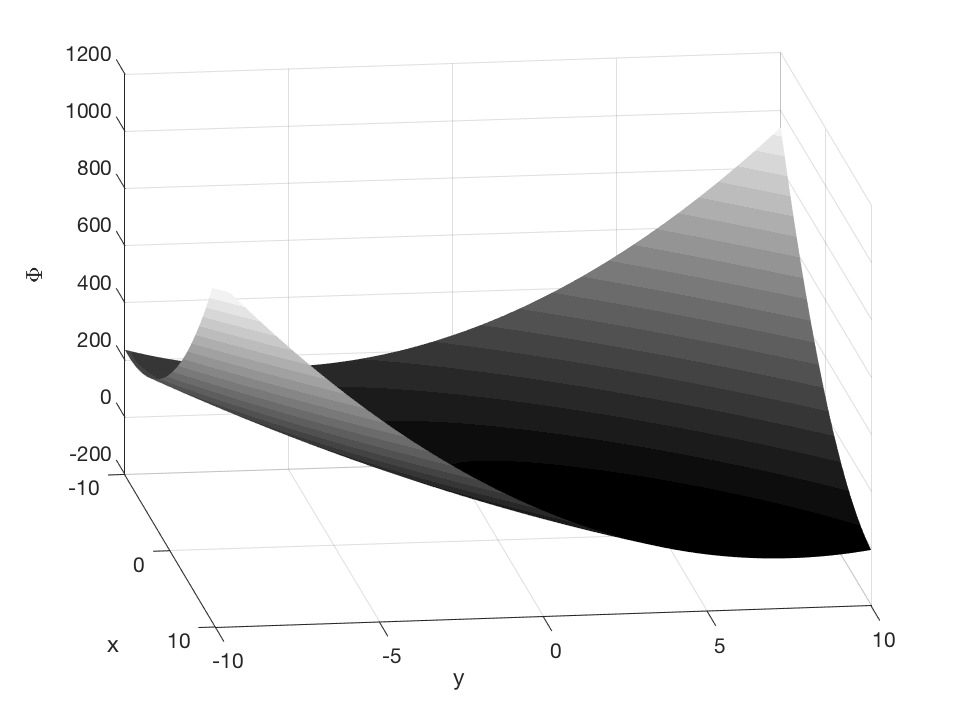
\includegraphics[width=\textwidth]{fig-esempio-energia-sistema}
         \caption{Prima.}
     \end{subfigure}
     \hfill
     \begin{subfigure}[b]{0.45\textwidth}
         \centering
         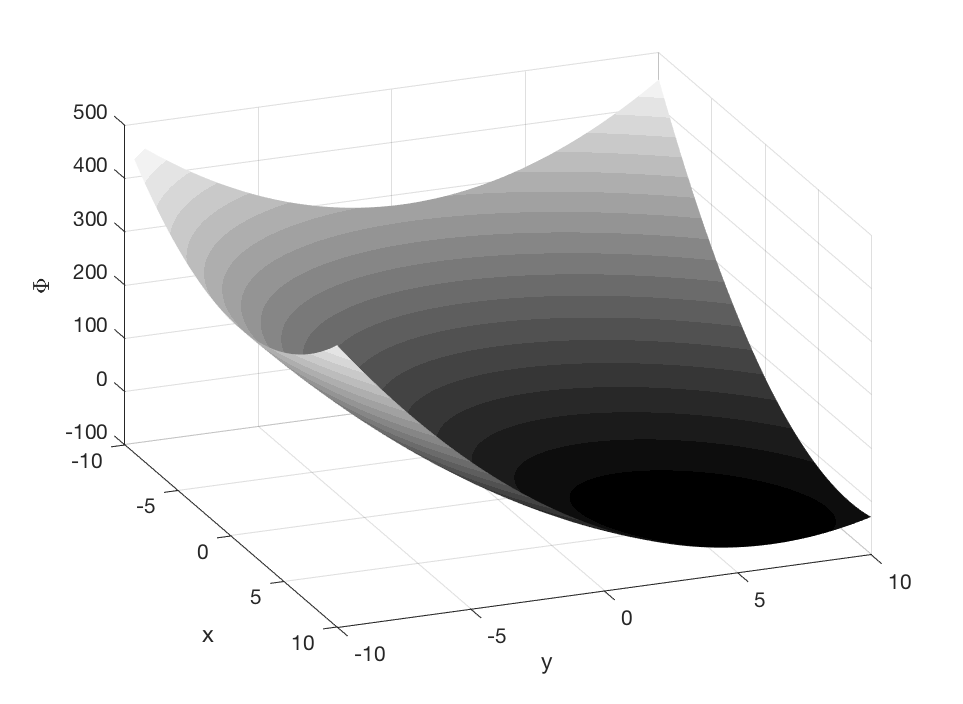
\includegraphics[width=\textwidth]{fig-esempio-energia-sistema-precond}
         \caption{Dopo.}
     \end{subfigure}
        \caption{Effetto del precondizionamento sull'energia del sistema.}
        \label{fig:effetto-precondizionamento}
\end{figure}

\begin{figure}[htpb]
     \centering
     \begin{subfigure}[b]{0.45\textwidth}
         \centering
         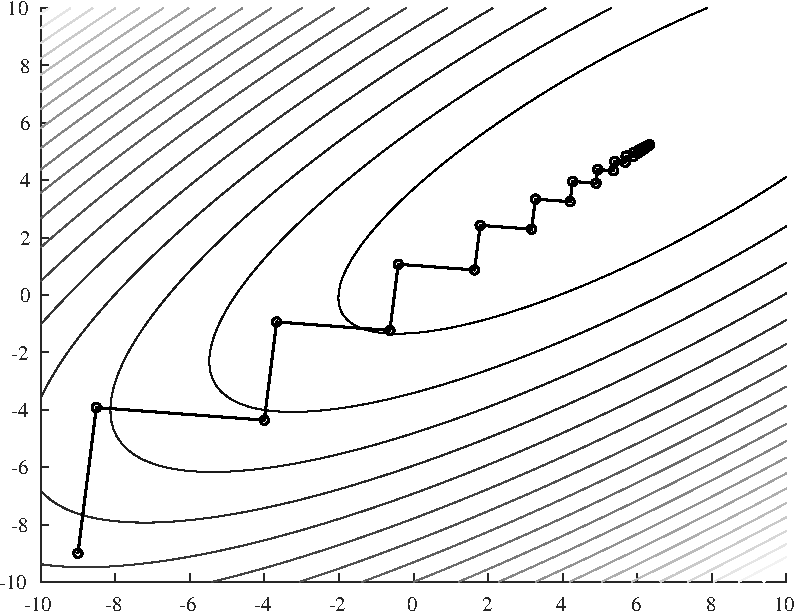
\includegraphics[width=\textwidth]{fig-esempio-soluzione}
         \caption{Prima.}
     \end{subfigure}
     \hfill
     \begin{subfigure}[b]{0.45\textwidth}
         \centering
         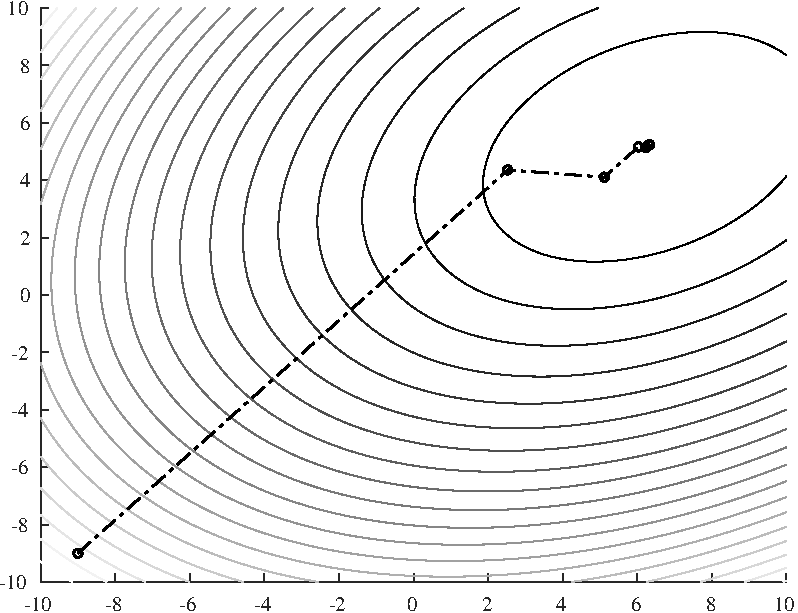
\includegraphics[width=\textwidth]{fig-esempio-soluzione-precond}
         \caption{Dopo.}
     \end{subfigure}
        \caption{Confronto sul numero di iterazioni necessarie con e senza precondizionamento.}
        \label{fig:effetto-precondizionamento-soluzione}
\end{figure}
% NB questi plot stanno nel file lab07_es01.m del laboratorio di matematica numerica

\begin{algo}
	inizializza $\x^{(0)}$\;
	calcola $\mathbf{r}^{(0)}$\;
	\For{$k=0,1,2,\dotsc$}{
		calcola il parametro ottimale di accelerazione $\alpha _{k} =\frac{\left[\mathbf{r}^{(k)}\right]^{T}\mathbf{r}^{(k)}}{\left[\mathbf{r}^{(k)}\right]^{T}\textcolor[rgb]{0.61,0.61,0.61}{A\ }\textcolor[rgb]{0.61,0.61,0.61}{\mathbf{r}}\textcolor[rgb]{0.61,0.61,0.61}{^{(k)}}}$\;
		aggiorna $\x^{( k+1)} =\x^{(k)} +\alpha _{k}\mathbf{r}^{(k)}$\;
		aggiorna $\mathbf{r}^{( k+1)} =\mathbf{r}^{(k)} -\alpha _{k}\textcolor[rgb]{0.61,0.61,0.61}{A\ }\textcolor[rgb]{0.61,0.61,0.61}{\mathbf{r}}\textcolor[rgb]{0.61,0.61,0.61}{^{\textcolor[rgb]{0.61,0.61,0.61}{(}\textcolor[rgb]{0.61,0.61,0.61}{k}\textcolor[rgb]{0.61,0.61,0.61}{)}}}$\;
		\If{criterio di arresto}{
			termina algoritmo\;
		}
	}
	\caption{Algoritmo del gradiente non precondizionato}
\end{algo}

\begin{algo}
	inizializza $\x^{(0)}$\;
	calcola $\mathbf{r}^{(0)}$\;
	\For{$k=0,1,2,\dotsc $}{
		calcola il residuo precondizionato $P\mathbf{z}^{(k)} =\mathbf{r}^{(k)}$\;
		calcola il parametro ottimale di accelerazione $\alpha _{k} =\frac{\left[\mathbf{z}^{(k)}\right]^{T}\mathbf{r}^{(k)}}{\left[\mathbf{z}^{(k)}\right]^{T}\textcolor[rgb]{0.61,0.61,0.61}{A\ }\mathbf{\textcolor[rgb]{0.61,0.61,0.61}{z}}\textcolor[rgb]{0.61,0.61,0.61}{^{(k)}}}$\;
		aggiorna $\x^{( k+1)} =\x^{(k)} +\alpha _{k}\mathbf{z}^{(k)}$\;
		aggiorna $\mathbf{r}^{( k+1)} =\mathbf{r}^{(k)} -\alpha _{k}\textcolor[rgb]{0.61,0.61,0.61}{A\ }\mathbf{\textcolor[rgb]{0.61,0.61,0.61}{z}}\textcolor[rgb]{0.61,0.61,0.61}{^{\textcolor[rgb]{0.61,0.61,0.61}{(}\textcolor[rgb]{0.61,0.61,0.61}{k}\textcolor[rgb]{0.61,0.61,0.61}{)}}}$\;
		\If{criterio di arresto}{
			termina algoritmo\;
		}
	}
	\caption{Algoritmo del gradiente precondizionato, $P$ SDP}
\end{algo}

\begin{theorem}
[Convergenza metodo del gradiente]
\index{convergenza!metodo del gradiente}
Siano $A$ e $P$ due matrici SDP. Allora il metodo del gradiente (con o senza precondizionatore) converge per ogni scelta di $\x^{(0)}$, e inoltre la successione delle iterate convergenti è monotona:
\begin{equation*}
\left\Vert \mathbf{e}^{( k+1)}\right\Vert _{A} \leqslant \left[\frac{K_{2}\left( P^{-1} A\right) -1}{K_{2}\left( P^{-1} A\right) +1}\right]\left\Vert \mathbf{e}^{(k)}\right\Vert _{A} ,\quad \forall k=0,1,2,\dotsc
\end{equation*}
dove $\Vert \cdot \Vert _{A}$ è la \textbf{norma dell'energia} definita come
\begin{equation*}
\Vert \mathbf{w}\Vert _{A} =\sqrt{\mathbf{w}^{T} A\mathbf{w}} \qquad \forall \mathbf{w} \in \mathbb{R}^{n}.
\end{equation*}
\end{theorem}
% \textit{[Lezione 9 (31-03-2020)]}

\textit{Osservazioni.}
\begin{itemize}
\item La velocità di convergenza è legata al rapporto
\begin{equation}
\frac{K_{2}\left( P^{-1} A\right) -1}{K_{2}\left( P^{-1} A\right) +1}.
\label{eq:termine-legato-velocita}
\end{equation}
\item Esso è sempre minore di $1$, e questo garantisce la convergenza del metodo:
\begin{equation*}
\left[\frac{K_{2}\left( P^{-1} A\right) -1}{K_{2}\left( P^{-1} A\right) +1}\right] < 1\ \ \Rightarrow \ \ \left\Vert \mathbf{e}^{(k)}\right\Vert _{A}\xrightarrow{k\rightarrow \infty } 0.
\end{equation*}
\item Se $A$ è mal condizionata si ha
\begin{equation*}
K_{2} \gg 1\ \ \Rightarrow \ \ \frac{K_{2} -1}{K_{2} +1} \approx 1\ \ \Rightarrow \ \ \text{convergenza lenta}.
\end{equation*}
\item Il precondizionamento migliora la proprietà di convergenza. L'idea è di scegliere $P$ tale che \eqref{eq:termine-legato-velocita} sia il più piccolo possibile (o analogamente che $K_{2}\left( P^{-1} A\right)$ sia il più vicino a $1$).
Ovviamente bisogna tenere conto del fatto che per ogni iterazione dobbiamo risolvere $P\mathbf{z}^{(k)} =\mathbf{r}^{(k)}$.
Si ha quindi un \textit{trade-off}\footnote{``There are no solutions. There are only trade-offs.'' -- Thomas Sowell}
in cui bisogna bilanciare due aspetti positivi opposti:

\begin{figure}[htpb]
	\centering
	\tikzset{every picture/.style={line width=0.75pt}} %set default line width to 0.75pt

	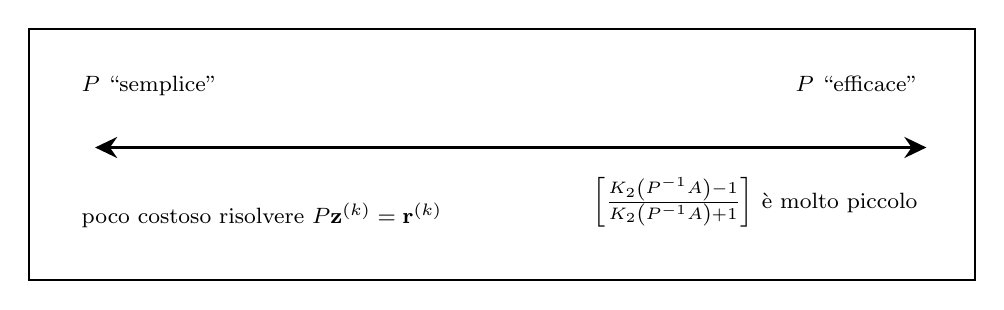
\begin{tikzpicture}[x=0.75pt,y=0.75pt,yscale=-1,xscale=1]
	%uncomment if require: \path (0,155); %set diagram left start at 0, and has height of 155

	%Straight Lines [id:da6554701139004233]
	\draw    (77,70) -- (471.5,70) ;
	\draw [shift={(474.5,70)}, rotate = 180] [fill={rgb, 255:red, 0; green, 0; blue, 0 }  ][line width=0.08]  [draw opacity=0] (10.72,-5.15) -- (0,0) -- (10.72,5.15) -- (7.12,0) -- cycle    ;
	\draw [shift={(74,70)}, rotate = 0] [fill={rgb, 255:red, 0; green, 0; blue, 0 }  ][line width=0.08]  [draw opacity=0] (10.72,-5.15) -- (0,0) -- (10.72,5.15) -- (7.12,0) -- cycle    ;
	%Shape: Rectangle [id:dp8278085571849905]
	\draw   (42,12.77) -- (497.81,12.77) -- (497.81,134) -- (42,134) -- cycle ;

	% Text Node
	\draw (66,34) node [anchor=north west][inner sep=0.75pt]  [font=\footnotesize] [align=left] {$P$ ``semplice''};
	% Text Node
	\draw (410,34) node [anchor=north west][inner sep=0.75pt]  [font=\footnotesize] [align=left] {$P$ ``efficace''};
	% Text Node
	\draw (66,95.5) node [anchor=north west][inner sep=0.75pt]  [font=\footnotesize] [align=left] {poco costoso risolvere $P\mathbf{z}^{(k)} =\mathbf{r}^{(k)}$};
	% Text Node
	\draw (312,83) node [anchor=north west][inner sep=0.75pt]  [font=\footnotesize] [align=left] {$\left[\frac{K_{2}\left( P^{-1} A\right) -1}{K_{2}\left( P^{-1} A\right) +1}\right]$ è molto piccolo};


	\end{tikzpicture}
\end{figure}
\FloatBarrier

\end{itemize}

\textbf{NB.}
Osserviamo che due vettori del residuo consecutivi nel metodo del gradiente non precondizionato (ma vale anche in quello precondizionato) soddisfano la seguente proprietà:
\begin{equation}
\left(\mathbf{r}^{( k+1)}\right)^{T}\mathbf{r}^{(k)} = 0,
\label{eq:prop-ortogonalita-gradiente}
\end{equation}
ovvero i valori del residuo sono \textit{a due a due ortogonali}. Quindi, ad ogni passo $k$ la nuova soluzione $\x^{( k+1)}$ è ottimale rispetto alla direzione di discesa $\mathbf{r}^{(k)}$.

\textit{Dimostrazione} di \eqref{eq:prop-ortogonalita-gradiente}. Ci ricordiamo la relazione di $\mathbf{r}^{( k+1)}$ che compare nell'algoritmo del gradiente e il valore di $\alpha _{k}$ \eqref{eq:alpha-ottimale-metodo-gradiente}:
\begin{equation*}
\mathbf{r}^{( k+1)} =\mathbf{r}^{(k)} -\alpha _{k} A\mathbf{r}^{(k)} ,\qquad \alpha _{k} =\frac{\left[\mathbf{r}^{(k)}\right]^{T}\mathbf{r}^{(k)}}{\left[\mathbf{r}^{(k)}\right]^{T} A\mathbf{r}^{(k)}} .
\end{equation*}
Calcoliamo il prodotto direttamente:
\begin{align*}
	\left(\mathbf{r}^{( k+1)}\right)^{T}\mathbf{r}^{(k)} & =\left(\mathbf{r}^{(k)} -\alpha _{k} A\mathbf{r}^{(k)}\right)^{T}\mathbf{r}^{(k)}                                                                                                                                         &                        \\
	                                                      & =\left(\left[\mathbf{r}^{(k)}\right]^{T} -\alpha _{k}\left[\mathbf{r}^{(k)}\right]^{T} A^{T}\right)\mathbf{r}^{(k)}                                                                                                       & \text{(trasposizione)} \\
	                                                      & =\left[\mathbf{r}^{(k)}\right]^{T}\mathbf{r}^{(k)} -\alpha _{k}\left[\mathbf{r}^{(k)}\right]^{T} A\mathbf{r}^{(k)}                                                                                                       & \text{(per simmetria)} \\
	                                                      & =\left[\mathbf{r}^{(k)}\right]^{T}\mathbf{r}^{(k)} -\frac{\left[\mathbf{r}^{(k)}\right]^{T}\mathbf{r}^{(k)}}{\left[\mathbf{r}^{(k)}\right]^{T} A\mathbf{r}^{(k)}}\left[\mathbf{r}^{(k)}\right]^{T} A\mathbf{r}^{(k)} & \text{(per ipotesi)}   \\
	                                                      & =\left[\mathbf{r}^{(k)}\right]^{T}\mathbf{r}^{(k)} -\left[\mathbf{r}^{(k)}\right]^{T}\mathbf{r}^{(k)}                                                                                                                    &                        \\
	                                                      & =0 \qed
\end{align*}

Notiamo tuttavia che \textit{non è garantito} che $\x^{( k+1)}$ sia ottimale rispetto a tutti i residui calcolati ai passi precedenti a $k$, ad esempio tutti i passi $j=0,\dotsc ,k-1$:
\begin{equation*}
\left[\mathbf{r}^{( k+1)}\right]^{T}\mathbf{r}^{(k)} =0,\quad\text{ma} \quad\left[\mathbf{r}^{( k+1)}\right]^{T}\mathbf{r}^{(j)} \neq 0,\quad j=0,\dotsc ,k-1.
\end{equation*}
Infatti, il metodo del gradiente non tiene traccia di tutte le direzioni precedenti, ma solo di quella immediatamente precedente.

\section{Metodo del gradiente coniugato}
\index{metodo!del gradiente coniugato}
È possibile modificare la direzione di discesa in modo da garantire un qualche criterio di \textit{ottimalità}?
Questa è l'idea che sta alla base del metodo del gradiente coniugato (GC o CG)\footnote{che ``è la Ferrari dei metodi iterativi''.}.
In particolare, dato un metodo iterativo
\begin{equation*}
\x^{( k+1)} =\x^{(k)} +\alpha _{k}\mathbf{p}^{(k)}
\end{equation*}
vogliamo scegliere direzioni di discesa che costituiscano una successione ottimale di vettori $\mathbf{p}^{(k)}$.
\begin{definition}
[Vettori $A$-coniugati]
Sia $A$ SDP fissata.
Due vettori $\mathbf{w} ,\mathbf{v} \in \mathbb{R}^{n}$ si dicono $A$-coniugati (o $A$-ortogonali) se
\begin{equation*}
\mathbf{w}^{T} A\ \mathbf{v} =0\quad\text{cioè} \quad ( A\mathbf{w})^{T}\mathbf{v} =0.
\end{equation*}
\end{definition}
\textit{Osservazioni.}
\begin{itemize}
\item Simmetria: $0=\left(\mathbf{w}^{T} A\ \mathbf{v}\right)^{T} =\mathbf{v}^{T} A^{T}\mathbf{w} =\mathbf{v}^{T} A\ \mathbf{w}$.
\item Annullamento: $\mathbf{v}^{T} A\mathbf{v} =0\ \Rightarrow \ \mathbf{v} =\mathbf{0}$.
\end{itemize}

\subsection{Scelta della direzione di discesa}
Scegliamo la seguente successione di vettori:
\begin{equation}
\begin{cases}
\mathbf{p}^{(0)} =\mathbf{r}^{(0)}\\
\mathbf{p}^{( k+1)} =\mathbf{r}^{( k+1)} -\beta _{k}\mathbf{p}^{(k)}
\end{cases} \quad \beta _{k} =\frac{\left( A\mathbf{p}^{(k)}\right)^{T}\mathbf{r}^{( k+1)}}{\left( A\mathbf{p}^{(k)}\right)^{T}\mathbf{p}^{(k)}} \quad k=0,1,2,\dotsc
\label{eq:scelta-metodo-cg}
\end{equation}
\textbf{Proprietà.}

Si può dimostrare per induzione che con la scelta \eqref{eq:scelta-metodo-cg} si ha:
\begin{enumerate}
\item $\left[\mathbf{p}^{(j)}\right]^{T}\mathbf{r}^{( k+1)} =0 \quad \forall j=0,1,\dotsc ,k$

La soluzione $\x^{( k+1)}$ è ottimale rispetto a \textit{tutte} le direzioni di discesa precedenti $\mathbf{p}^{(0)} ,\mathbf{p}^{(1)} ,\mathbf{p}^{(2)} ,\dotsc ,\mathbf{p}^{(k)}$.
\item $\left[ A\mathbf{p}^{(j)}\right]^{T}\mathbf{p}^{( k+1)} =0 \quad \forall j=0,1,\dotsc ,k$

La direzione di discesa $\mathbf{p}^{( k+1)}$ è $A$-ortogonale rispetto a \textit{tutte} le direzioni $\mathbf{p}^{(0)} ,\mathbf{p}^{(1)} ,\mathbf{p}^{(2)} ,\dotsc ,\mathbf{p}^{(k)}$. Ad ogni passo, l'algoritmo esplora e minimizza una direzione nuova, mai usata prima, tralasciando lo spazio già precedentemente esplorato.
\item Combinando $(1)$ e $(2)$ al passo $n$-esimo si ha $\mathbf{r}^{(n)} =0$, ossia $\x^{(n)}$ \textit{è la soluzione esatta}\footnote{Mai notizia più buona fu data.}.
\end{enumerate}

Dimostriamo la proprietà $(3)$, lasciando $(1)$ e $(2)$ al lettore come esercizio.
Per la proprietà $(1)$, al passo $k=n-1$ si ha:
\begin{equation*}
\underbrace{\mathbf{r}^{(n)}}_{\in \mathbb{R}^{n}} \perp \mathbf{p}^{(0)} ,\mathbf{p}^{(1)} ,\dotsc ,\mathbf{p}^{( n-1)}.
\end{equation*}
Non è ancora possibile concludere che $\mathbf{r}^{(n)}$ è nullo in quanto ortogonale ad altri $n$ vettori, perché non sappiamo se gli altri $\mathbf{p}^{(k)}$ sono indipendenti.
Ma vedremo che questa proprietà è assicurata dalla $(2)$.
Prendiamo la combinazione lineare dei vettori precedenti e poniamola uguale a $0$: vogliamo dimostrare che ciò implica necessariamente che tutti i coefficienti sono nulli:
\begin{equation*}
a_{0}\mathbf{p}^{(0)} +a_{1}\mathbf{p}^{(1)} +\dotsc +a_{n-1}\mathbf{p}^{( n-1)} =0\xrightarrow{\text{?}} a_{i} =0\quad\forall i=0,\dotsc ,n-1.
\end{equation*}
Moltiplichiamo a destra e sinistra per $\left( A\mathbf{p}^{(0)}\right)^{T}$:
\begin{equation*}
a_{0}\underbrace{\left( A\mathbf{p}^{(0)}\right)^{T}\mathbf{p}^{(0)}}_{ >0\text{ se }\mathbf{p}^{(0)} \neq 0} +a_{1}\underbrace{\left( A\mathbf{p}^{(0)}\right)^{T}\mathbf{p}^{(1)}}_{=0\ \text{per} \ (2)} +\dotsc +a_{n-1}\left( A\mathbf{p}^{(0)}\right)^{T}\mathbf{p}^{( n-1)} =0 \ \ \Rightarrow \ \ a_{0} =0.
\end{equation*}
Analogamente moltiplicando per $\left( A\mathbf{p}^{(1)}\right)^{T}$ si ricava $a_{1} =0$ e così via. Infine si ottiene $a_{i} =0\ \ \forall i$, ovvero che tutti i $\mathbf{p}^{(i)}$ sono linearmente indipendenti. \textqed

\subsection{Scelta del parametro di accelerazione}
Ripercorrendo gli stessi passi della sezione \eqref{sez:metodo-del-gradiente} sulla minimizzazione del funzionale $\Phi ( \cdot )$, valutato questa volta in $\x^{( k+1)} =\x^{(k)} +\alpha _{k}\mathbf{p}^{(k)}$, troviamo:
\begin{equation*}
\alpha_{k} =\frac{\left[\mathbf{p}^{(k)}\right]^{T}\mathbf{r}^{(k)}}{\left[\mathbf{p}^{(k)}\right]^{T} A\ \mathbf{p}^{(k)}}.
\end{equation*}
Riassumiamo il gradiente coniugato in pseudocodice: \\
\begin{algo}
	inizializza $\x^{(0)}$\;
	calcola $\mathbf{r}^{(0)} =\mathbf{b} -A\x^{(0)}$\;
	inizializza $\mathbf{p}^{(0)} =\mathbf{r}^{(0)}$\;
	\For{$k=0,1,2,\dotsc $}{
		calcola il parametro $\alpha _{k} =\frac{\left[\mathbf{p}^{(k)}\right]^{T}\mathbf{r}^{(k)}}{\left[\mathbf{p}^{(k)}\right]^{T} A\ \mathbf{p}^{(k)}}$\;
		aggiorna $\x^{( k+1)} =\x^{(k)} +\alpha _{k}\mathbf{p}^{(k)}$\;
		aggiorna $\mathbf{r}^{( k+1)} =\mathbf{r}^{(k)} -\alpha _{k} A\mathbf{p}^{(k)}$\;
		calcola il parametro $\beta _{k} =\frac{\left( A\mathbf{p}^{(k)}\right)^{T}\mathbf{r}^{( k+1)}}{\left( A\mathbf{p}^{(k)}\right)^{T}\mathbf{p}^{(k)}}$\;
		aggiorna $\mathbf{p}^{( k+1)} =\mathbf{r}^{( k+1)} -\beta _{k}\mathbf{p}^{(k)}$\;
		\If{criterio di arresto}{
			termina algoritmo\;
		}
	}
	\caption{Algoritmo del metodo del gradiente coniugato, non precondizionato}
\end{algo}
\index{algoritmo!gradiente coniugato}
\begin{theorem}
[Convergenza del metodo GC]
Sia $A$ una matrice SDP in aritmetica esatta.
Allora il metodo GC converge alla soluzione esatta di $A \x = \mathbf b$ in al più $n$ passi. Inoltre, per ogni iterazione $k=0,\dotsc ,n$, l'errore $\mathbf{e}^{(k)}$ è ortogonale alla direzione $\mathbf{p}^{(j)} \quad j=0,\dotsc ,k-1$ e
\begin{equation*}
\left\Vert \mathbf{e}^{(k)}\right\Vert _{A} \leqslant \left[\frac{2c^{k}}{1+c^{2k}}\right]\left\Vert \mathbf{e}^{(0)}\right\Vert _{A} \quad\text{con} \quad c=\frac{\sqrt{K_{2}(A)} -1}{\sqrt{K_{2}(A)} +1}.
\end{equation*}
\label{thm:convergenza-metodo-cg}
\end{theorem}
\textit{Osservazioni.}
\begin{itemize}
\item Se $A$ è SDP, allora $K_{2}(A) =\frac{\lambda _{\text{max}}(A)}{\lambda _{\text{min}}(A)}$.
%\item In aritmetica esatta abbiamo la certezza che l'algoritmo termini dopo al più $n$ passi restituendo la soluzione esatta. % l'hai già detto
\item Come per il metodo del gradiente la convergenza è monotona, e in particolare la sua velocità dipende da $\sqrt{K_{2}(A)}$.
\end{itemize}

Scriviamo ora la versione precondizionata del gradiente coniugato: \\
\begin{algo}
	inizializza $\x^{(0)}$\;
	calcola $\mathbf{r}^{(0)} =\mathbf{b} -A\x^{(0)}$\;
	risolvi $P\mathbf{z}^{(0)} = \mathbf{r}^{(0)}$\;
	inizializza $\mathbf{p}^{(0)} = \mathbf{z}^{(0)}$\;
	\For{$k=0,1,2,\dotsc$}{
		calcola il parametro $\alpha _{k} =\frac{\left[\mathbf{p}^{(k)}\right]^{T}\mathbf{r}^{(k)}}{\left[\mathbf{p}^{(k)}\right]^{T} A\ \mathbf{p}^{(k)}}$\;
		aggiorna $\x^{( k+1)} =\x^{(k)} +\alpha _{k}\mathbf{p}^{(k)}$\;
		aggiorna $\mathbf{r}^{( k+1)} =\mathbf{r}^{(k)} -\alpha _{k} A\mathbf{p}^{(k)}$\;
		risolvi $P\mathbf{z}^{(k+1)} = \mathbf{r}^{(k+1)}$\;
		calcola il parametro $\beta _{k} =\frac{\left( A\mathbf{p}^{(k)}\right)^{T}\mathbf{z}^{(k+1)}}{\left( A\mathbf{p}^{(k)}\right)^{T}\mathbf{p}^{(k)}}$\;
		aggiorna $\mathbf{p}^{( k+1)} =\mathbf{z}^{(k+1)} -\beta _{k}\mathbf{p}^{(k)}$\;
		\If{criterio di arresto}{
			termina algoritmo\;
		}
	}
	\caption{Algoritmo del metodo del gradiente coniugato, precondizionato}
\end{algo}
\index{algoritmo!gradiente coniugato}
Per esso vale lo stesso teorema di convergenza \ref{thm:convergenza-metodo-cg}, con
\begin{equation*}
c=\frac{\sqrt{K_{2}\left( P^{-1} A\right)} -1}{\sqrt{K_{2}\left( P^{-1} A\right)} +1}.
\end{equation*}
\section{Criteri di arresto}

I criteri di arresto non dipendono nello specifico dai metodi che stiamo utilizzando. Fissiamo una tolleranza $\operatorname{TOL}$, ovvero una quantità decisa dall'utente, che la sceglie in base a quanta precisione desidera nel calcolo della soluzione.
%$Non è necessariamente il più piccolo numero del calcolatore (potremmo aver bisogno di tolleranza $10^{-6}$ e non $10^{-16}$). % bah
Più piccola è $\operatorname{TOL}$, più iterazioni l'algoritmo necessita per convergere: dobbiamo trovare un equilibrio, un trade-off, tra quanto vogliamo essere accurati e quante iterazioni siamo disposti ad aspettare.
\begin{enumerate}
\item \textbf{Criterio sul residuo.} Arrestiamo il ciclo quando
\begin{equation*}
\frac{\left\Vert \mathbf{r}^{( k+1)}\right\Vert }{\Vert \mathbf{b}\Vert } \leqslant \operatorname{TOL}.
\end{equation*}
\item \textbf{Criterio sull'incremento.} Arrestiamo il ciclo quando
\begin{equation*}
\left\Vert \x^{( k+1)} -\x^{(k)}\right\Vert \leqslant \operatorname{TOL}.
\end{equation*}
\item \textbf{Criterio di controllo.} Arrestiamo il ciclo dopo $n_{\text{max}}$ iterazioni.
\end{enumerate}

\textit{Osservazioni.}
\begin{itemize}
\item I criteri (1) e (2) agiscono in funzione della \textit{qualità della soluzione}, mentre (3) è un criterio di emergenza.
\item Di norma si sceglie di usare uno tra i primi due criteri, abbinati sempre al terzo. Infatti ci sono matrici che convergono lentissimamente, che hanno bisogno di molte iterazioni per raggiungere un risultato soddisfacente.
\item Ogni iterazione di Gauss-Seidel costa $n^{2}$ operazioni. Dopo $n$ iterazioni, il costo complessivo diventa $n^{3}$, esattamente il costo di una fattorizzazione con metodo diretto. Per tutti i problemi in cui non c'è problema di memoria limitata e quindi possiamo scegliere fra metodi diretti e iterativi, il metodo iterativo è molto più conveniente nella misura in cui andiamo a usare un criterio di arresto in meno di $n$ operazioni. Quindi $n_{\text{max}} \approx n$. Se abbiamo troppo poco spazio, i metodi iterativi sono d'obbligo.
\item Il criterio (2) lascia proseguire l'algoritmo fintanto che fra l'iterazione $(k)$ e l'iterazione $( k+1)$ c'è sufficiente progresso. Se $\x^{(k)}$ e $\x^{( k+1)}$ sono molto vicine, significa che l'algoritmo sta stagnando.
\item Un criterio si dice \textbf{affidabile} se nel momento in cui si verifica la condizione, abbiamo la garanzia che anche l'errore (normalizzato) sia minore della tolleranza moltiplicata per una costante.
\end{itemize}
\subsection{Criterio sul residuo}

Controlliamo l'affidabilità del criterio sul residuo. L'algoritmo si arresta quando si verifica:
\begin{equation}
\frac{\left\Vert \mathbf{r}^{(k)}\right\Vert }{\Vert \mathbf{b}\Vert } \leqslant \operatorname{TOL}.
\label{eq:criterio-residuo}
\end{equation}
Dobbiamo verificare se valga la seguente implicazione, come notato nelle osservazioni:
\begin{equation*}
\frac{\left\Vert \mathbf{r}^{(k)}\right\Vert }{\Vert \mathbf{b}\Vert } \leqslant \operatorname{TOL} \ \ \overset{?}{\Rightarrow } \ \ \frac{\left\Vert \mathbf{e}^{(k)}\right\Vert }{\Vert \x\Vert } =\frac{\left\Vert \x -\x^{(k)}\right\Vert }{\Vert \x\Vert } \leqslant C\ \operatorname{TOL}.
\end{equation*}
A tal proposito, ricordiamo il teorema di stabilità dei sistemi lineari \ref{thm:teorema-di-stabilita}:
\begin{equation*}
\frac{\left\Vert \x -\tilde{\x}\right\Vert }{\Vert \x\Vert } \leqslant K_{2}(A)\frac{\left\Vert \mathbf{b} -A\tilde{\x}\right\Vert }{\Vert \mathbf{b}\Vert }
\end{equation*}
Prendendo $\tilde{\x} =\x^{(k)}$ e ricordando che $\mathbf{b} -A\x^{(k)} =\mathbf{r}^{(k)}$, l'enunciato del teorema diventa:
\begin{equation}
\frac{\left\Vert \x -\x^{(k)}\right\Vert }{\Vert \x\Vert } \leqslant K_{2}(A)\frac{\left\Vert \mathbf{r}^{(k)} \ \right\Vert }{\Vert \mathbf{b}\Vert } \leqslant K_{2}(A) \ \operatorname{TOL}.
\label{eq:criterio-residuo2}
\end{equation}
Quindi il criterio d'arresto sul residuo \eqref{eq:criterio-residuo} è affidabile solo se la matrice è ben condizionata. Nel caso usassimo un precondizionatore, bisogna sostituire il criterio con il seguente:
\begin{equation*}
\frac{\left\Vert P^{-1}\mathbf{r}^{(k)}\right\Vert }{\left\Vert P^{-1}\mathbf{r}^{(0)}\right\Vert } \leqslant \operatorname{TOL} \quad \text{oppure analogamente} \quad \frac{\left\Vert \mathbf{z}^{(k)}\right\Vert }{\left\Vert \mathbf{z}^{(0)}\right\Vert } \leqslant \operatorname{TOL},
\end{equation*}
in tal caso la \eqref{eq:criterio-residuo2} diventa:
\begin{equation*}
\frac{\left\Vert \x -\x^{(k)}\right\Vert }{\Vert \x\Vert } \leqslant K_{2}\left( P^{-1} A\right) \ \operatorname{TOL}.
\end{equation*}
\subsection{Criterio sull'incremento}

Studiamo ora l'affidabilità del criterio sull'incremento:
\begin{equation}
\frac{\left\Vert \x^{( k+1)} -\x^{(k)}\right\Vert }{\left\Vert \x^{( k+1)}\right\Vert } \leqslant \operatorname{TOL}.
\label{eq:criterio-incremento}
\end{equation}
Bisogna verificare la seguente implicazione:
\begin{equation*}
\frac{\left\Vert \x^{( k+1)} -\x^{(k)}\right\Vert }{\left\Vert \x^{( k+1)}\right\Vert } \leqslant \operatorname{TOL} \ \ \overset{?}{\Rightarrow } \ \ \frac{\left\Vert \mathbf{e}^{(k)}\right\Vert }{\Vert \x\Vert } =\frac{\left\Vert \x -\x^{(k)}\right\Vert }{\Vert \x\Vert } \leqslant C\ \operatorname{TOL}.
\end{equation*}
A tal proposito, ricordiamo:
\begin{align*}
\x^{( k+1)} & =B\x^{(k)} +\mathbf{g} & \text{(forma generale)}\\
\x & =B\x +\mathbf{g} & \text{(consistenza)}\\
\x^{( k+1)} -\x & =B(\x^{(k)} -\x). & \text{(differenza)}
\end{align*}
L'errore $k$-esimo si può scrivere come:
\begin{align*}
  \left\Vert \mathbf{e}^{(k)}\right\Vert =\left\Vert \x^{(k)} -\x\right\Vert & =\left\Vert \x^{(k)} -\x^{( k+1)} +\x^{( k+1)} -\x\right\Vert                                             &                           \\
  & \leqslant \left\Vert \x^{( k+1)} -\x^{(k)}\right\Vert +\left\Vert \x^{( k+1)} -\x\right\Vert              & \text{(dis. triangolare)} \\
  & \leqslant \left\Vert \x^{( k+1)} -\x^{(k)}\right\Vert +\Vert B\Vert \ \left\Vert \x^{(k)} -\x\right\Vert. & \text{(per quanto detto)}
\end{align*}
Portiamo a sinistra e dividiamo per $1-\Vert B\Vert $:
\begin{align*}
( 1-\Vert B\Vert )\left\Vert \x^{(k)} -\x\right\Vert  & \leqslant \left\Vert \x^{( k+1)} -\x^{(k)}\right\Vert \\
\underbrace{\left\Vert \x^{(k)} -\x\right\Vert }_{\left\Vert \mathbf{e}^{(k)}\right\Vert } & \leqslant \frac{1}{1-\Vert B\Vert }\left\Vert \x^{( k+1)} -\x^{(k)}\right\Vert.
\end{align*}
Infine, ricordando la formula di rappresentazione dell'errore $\mathbf{e}^{( k+1)} =B\mathbf{e}^{(k)}$:
\begin{align*}
\left\Vert \x^{( k+1)} -\x\right\Vert  & =\left\Vert \mathbf{e}^{( k+1)}\right\Vert  & \\
 & =\left\Vert B\mathbf{e}^{(k)}\right\Vert  & \text{(formula di rappr. dell'errore)}\\
 & \leqslant \Vert B\Vert \ \left\Vert \mathbf{e}^{(k)}\right\Vert  & \text{(proprietà della norma)}\\
 & \leqslant \frac{\Vert B\Vert }{1-\Vert B\Vert }\left\Vert \x^{( k+1)} -\x^{(k)}\right\Vert.  & \text{(per quanto appena trovato)}
\end{align*}
Otteniamo infine:
\begin{equation}
\left\Vert \x -\x^{( k+1)}\right\Vert \leqslant \frac{\Vert B\Vert }{1-\Vert B\Vert } \ \left\Vert \x^{( k+1)} -\x^{(k)}\right\Vert.
\label{eq:criterio-incremento2}
\end{equation}

Poiché il metodo è convergente si ha $\rho (B) < 1$, quindi $\Vert B\Vert < 1$. Il criterio è quindi affidabile. La \eqref{eq:criterio-incremento2} si può anche riscrivere come
\begin{equation*}
\left\Vert \x -\x^{( k+1)}\right\Vert \leqslant \left[\frac{1}{1-\rho (B)}\right]\left\Vert \x^{( k+1)} -\x^{(k)}\right\Vert.
\end{equation*}
Quindi se $\Vert B\Vert $ è molto vicina a $1$, cioè se $A$ è mal condizionata, la differenza tra l'errore vero e quello che sappiamo misurare diventa molto grande e quindi dà poche informazioni.
